\documentclass{article}

\usepackage{amstext}
\usepackage{amsmath,amsthm,amsfonts,amssymb}
\usepackage{booktabs} % for professional tables
\usepackage{bm}

\usepackage[T1, T2A]{fontenc}    % use 8-bit T1 fonts
\usepackage[utf8]{inputenc} % allow utf-8 input
\usepackage[english, russian]{babel}

\usepackage{float}
\usepackage{fontawesome}
\usepackage{geometry}
\usepackage{graphicx}
\usepackage{hyperref}       % hyperlinks
%\usepackage{lmodern}
\usepackage{mathtools}
\usepackage{microtype}      % microtypography
\usepackage{multirow}
\usepackage{nicefrac}       % compact symbols for 1/2, etc.
\usepackage{subfigure}
%\usepackage{times}
\usepackage{url}            % simple URL typesetting

\newcommand{\theHalgorithm}{\arabic{algorithm}}
\newcommand{\norm}[1]{\left\lVert#1\right\rVert}

\geometry{
    a4paper,
    total={160mm,237mm},
    left=25mm,
    top=30mm,
}
\setlength{\parindent}{0em}
\setlength{\parskip}{0.5em}
\renewcommand{\baselinestretch}{1.5}

\newtheorem{theorem}{Theorem}

\begin{document}
% ToDo: check everything with grammarly
% ToDo: probably add more citations where they are needed

\begin{titlepage}
\begin{center}
    \selectlanguage{russian}
	\selectlanguage{english}

    \large

	{\bfseries NATIONAL RESEARCH UNIVERSITY \\ <<HIGHER SCHOOL OF ECONOMICS>>}

	{\bf\textit{Faculty of Computer Science}}

	\bigskip
	\bigskip

	%Mihail Solotchii \\ % ToDo: should it be presented twice?

	\bigskip
	\bigskip

    \selectlanguage{russian}
    \textbf{Исследование свойств одномодельных методов оценки неопределенности на крупномасштабных задачах}

    \bigskip
    \bigskip

    \selectlanguage{english}
	{\bfseries Investigation of the behavior of single-model uncertainty estimation approaches on large-scale tasks}

    \bigskip
    \bigskip

    Qualification paper – Master of Science Dissertation 

    Field of study 01.04.02 <<Applied Mathematics and Informatics>>

    Program: <<Data Science>>

    \bigskip
    \bigskip

    \begin{flushleft}
        Student \\
        \underline{Mihail Solotchii } \\
    \end{flushleft}

    \begin{flushright}
        Supervisor \\
        \underline{ Artem Babenko} \\
    \end{flushright}

    \bigskip
    \bigskip

    \begin{flushright}
        Consultant \\ % ToDo: is it ok to write like that?
        \underline{ Andrey Malinin} \\
    \end{flushright}

    \bigskip
    \bigskip

	\vspace{\fill}
	Moscow, 2021
\end{center}
\end{titlepage}

\newpage

\selectlanguage{english}
\selectlanguage{russian}

\newpage
\thispagestyle{empty}
\begin{abstract}
Методы оценки неопределенности помогают моделям машинного обучения понимать, в каких ситуациях их предсказания будут ненадежными.
Имея возможность предсказывать надёжность предсказаний модели, мы можем построить более безопасную систему прогнозов посредством отказа от предсказаний и передачи объектов для распознавания другому алгоритму.
Стандартное предположение относительно данных для предсказания такое, что эти данные приходят из того же вероятностного распределения, что и обучающие данные.
На практике это условие не всегда соблюдается, и такие данные являются источником ошибочных предсказаний для широкого класса моделей машинного обучения.
Мы хотим детектировать такие примеры и применяем методы оценки эпистемической неопределенности для детекции объектов не из обучающего распределения.
Мы исследуем некоторые методы оценки неопределенности с целью понять, насколько они масштабируемы и каков механизм их работы.
Мы видим что простые подходы, такие как максимальный логит и энтропия софтмакса так же хорошо работают на задаче детекции примеров не из распределения, как и более дорогостоящие методы, такие как глубокие ансамбли.
Мы показываем связь между различными методами оценки неопределенности между собой и с методами, основанными на близости представлений в некотором латентном пространстве.
Мы предлагаем новый метод для оценки неопределенности и показываем, что его оценки коррелируют с похожестью объекта на обучающие объекты.
\end{abstract}

\selectlanguage{english}

\begin{abstract}
Methods of uncertainty estimation help models of machine learning understand in which cases their predictions would be unreliable.
With the ability to predict the unreliability of the model's predictions, we can design a safer AI system by rejecting predictions and passing the objects to another algorithm.
A standard assumption regarding data on the inference stage is that this data comes from the same probabilistic distribution as that on the training stage.
This condition is not always met in practice, and such data points cause many machine learning models to give wrong predictions.
We want to detect such data samples and use methods of epistemic uncertainty estimation for Out-of-Distribution (OoD) detection.
We investigate some methods of uncertainty estimation to understand whether they are scalable and how they work.
We see that simple approaches such as the maximal logit and the entropy of softmax work on par as OoD detectors as more expensive approaches such as the Deep Ensembles.
We show the connection between various approaches to uncertainty estimation and their connection with the methods that put objects in some latent space and interpret distance to training representations as a measure of epistemic uncertainty.
We propose a new simple method for uncertainty estimation and show that its uncertainty estimates correlate with the level similarity to the training objects.
\end{abstract}

\newpage

\setcounter{page}{1}
\tableofcontents
\newpage

\section{Introduction}
\label{introduction}
One of the standard assumptions made in machine learning theory is that the testing objects are drawn from the same probabilistic distribution as the training samples.
However, in practice, this condition is not always met.
Dataset shifts with various severity are common in real-world applications (e.g., images could be taken in different weather conditions, in different locations, or with some shooting defects).
The severity of the shifts usually correlates with the model's performance.
The less an object is related to the training distribution the less is the quality of the predictions.
The concept of uncertainty estimation (or quantification) is to find a measure that would correlate with the model's performance, which would tell how likely it is for the model to be mistaken on the particular input.
The model would be aware of its weaknesses, which can help design safe AI systems, which is very important for such areas as \textit{medical diagnostics} and \textit{self-driving vehicles}.

Sometimes values of some variables cannot be determined precisely.
It means there is uncertainty in the determination of the variable's value.
Usually, there are two types of uncertainty in machine learning.
The \textit{aleatoric} or \textit{data} uncertainty comes from the ambiguity in the training data (e.g., wrong labeling and class overlap).
The \textit{epistemic} or \textit{model} uncertainty comes from the lack of the model's knowledge about the specific input.
As the model was trained on the objects from a specific distribution, it has less knowledge about the objects from some shifted distribution or completely different distribution.
It means that modeling epistemic uncertainty can help detect dataset shifts. More generally, it helps to detect Out-of-Distribution (OoD) objects (i.e., objects drawn from a different probabilistic distribution than the training one).

% ToDo: come up with the final classification of the methods
There are various approaches to model epistemic uncertainty.
Some approaches try to model the posterior distribution over predictions given data and propose a decomposition of total uncertainty into \textit{aleatoric} and \textit{epistemic}.

This could be accomplished with the help of ensembles (e.g., Deep Ensembles \\ \cite{deep_ensembles}, Monte-Carlo dropout \cite{monte_carlo_dropout}), which are an approximation of the posterior distribution, or with a single network (called Prior Network \cite{prior_net}), which is trained to meet reasonable criteria that a true posterior would have.
These methods are theoretically justified, have a strong intuition behind them, and prove to work well.
Deep Ensembles are de facto a SotA approach for OoD detection.
However, they have several drawbacks that make them difficult to use in practical applications.
Ensembles are expensive to run on inference, while Prior Networks require an OoD set for training. Such a set could be inaccessible in some applications.

Another group of methods tries to put input objects into a latent space, where closeness to the In-Distribution (ID) representations would reflect the level of dataset shift. These include methods like Neural Gaussian Processes \cite{gp}, RBF networks \cite{duq, duq_improved}, k-Nearest Neighbours \cite{knn} in the embedding space.
% ToDo: finish this paragraph
% ToDo: say whether there is a consensus about this methods whether they should work
% ToDo: say about drawbacks

Moreover, a couple of other methods do not fall into any of the previously discussed groups.
They do not use distance-based intuition, require just a single model to run the inference, do not use any OoD sets during their training, and there is no consensus in the community about why these methods work.
These methods include the Evidential methods and some simple baselines like the maximal probability, maximal logit, the entropy of softmax.
% ToDo: finish this paragraph

This work has three main contributions:
\begin{enumerate}
\item We show the methods from the last group have similar performance to the SotA approach (i.e., Deep Ensembles) on close to the real world ImageNet dataset \cite{imagenet};
\item We show the Evidential setting proposed in the original paper \cite{evidential_classification} is not scalable as it was proposed and there are simple modifications which make it scale;
\item We show the hidden similarity between the methods from the last group and between them and the distance-based methods;
%\item We provide hypotheses that could answer the question <<Why do the methods from the last group work>> and provide experimental observations that align with the hypotheses.
\end{enumerate}
% ToDo: write what exactly are the hypotheses and what's the similarity

This work focuses on the classification task only. The experiments were done for image classification with standard computer vision architectures.
However, it is possible to reproduce these experiments on other data domains (like tabular data, for instance).

The following sections are arranged as follows: \\
The section <<\nameref{section:methods_description}>> explains the methods, which will be used in the experiment and analysis.
The section describes notation and all the necessary mathematics in detail.
Then goes the section <<\nameref{section:analysis}>>.
It provides a deeper understanding of the methods described earlier and shows some hidden similarities between the methods from the <<third group>>.
Then goes the <<\nameref{section:experiments}>> section, which provides the empirical results and describes details of experiments.
It is all finished with the <<\nameref{section:conclusion}>> section.

\section{Approaches to epistemic uncertainty estimation}
\label{section:methods_description}
This section is a detailed review of different approaches to epistemic uncertainty estimation. It is the basis for further analysis.

There is also some general notation that has to be introduced before the description of the methods starts.
The conventional notation for neural classification models is the following: the network $f_{\boldsymbol{\theta}}$ with the parameters $\boldsymbol{\theta}$ take an input object $\boldsymbol{x}$ and return logits i.e. the inputs of the softmax function, where they are transformed into predicted probabilities of the class labels
\begin{equation}
\mathrm{P}(y | \boldsymbol{x}) = \mathrm{SoftMax}(f_{\boldsymbol{\theta}}(\boldsymbol{x}))
\end{equation}

Sometimes, the softmax function is used, but ReLU, for instance, and still for simplicity, the inputs of such functions are called logits in some papers.

The vectors' names are highlighted in bold, and the scalars are not.
In the case of a discrete probability distribution, the large letter $\mathrm{P}$ is used to refer to the distribution (meaning the probability function), and in the case of a continuous distribution, the small letter $\mathrm{p}$ is used (meaning the probability density function).
The function $u(\boldsymbol{x})$ or for simplicity the $u$ letter this is the notation for uncertainty.
The letter $K$ denotes the number of classes, and the letter $c$ refers to some class label.

It is the standard notation that will be used in the following sections. All other notations used in one or a few methods will be introduced in the following sections.

\subsection{Bayesian definition of uncertainty}
Let us say have a family of classification models parameterized with a vector of parameters $\boldsymbol{\theta}$.
Then we have a training dataset $\mathcal{D} = \{\boldsymbol{x}_i, y_i\}_{i=1}^n$ consisting of input objects $\boldsymbol{x}_i$ and labels $y_i$.
With parameters $\boldsymbol{\theta^{*}}$ fixed we have a classification model which that takes an input $\boldsymbol{x}$ and returns a categorical probabilistic distribution over labels $\mathrm{P} (y | \boldsymbol{x}, \boldsymbol{\theta^{*}})$.
Having that model we can compute the training dataset likelihood $\mathrm{P} (\boldsymbol{Y}_{tr} | \boldsymbol{X}_{tr}, \boldsymbol{\theta^{*}}) = \prod\limits_{i=1}^n \mathrm{P} (y_i | \boldsymbol{x}_i, \boldsymbol{\theta^{*}})$.
If we consider a prior over the parameters, we then can compute the posterior distribution over the parameters given the training dataset $\mathcal{D}$ using the Bayes' theorem:
\begin{equation}
\mathrm{p} (\boldsymbol{\theta} | \mathcal{D}) = \mathrm{p} (\boldsymbol{\theta} | \boldsymbol{X}_{tr}, \boldsymbol{Y}_{tr}) = \frac{\mathrm{P} (\boldsymbol{Y}_{tr} | \boldsymbol{X}_{tr}, \boldsymbol{\theta}) \mathrm{p}(\boldsymbol{\theta})}{\int \mathrm{P} (\boldsymbol{Y}_{tr} | \boldsymbol{X}_{tr}, \boldsymbol{\theta}) \mathrm{p}(\boldsymbol{\theta}) d\boldsymbol{\theta}}
\end{equation}

Having the posterior distribution over parameters, one can compute the \textit{predictive posterior} distribution.
\begin{equation}
\mathrm{P} (y | \boldsymbol{x}, \mathcal{D}) = \int \mathrm{P} (y | \boldsymbol{x}, \boldsymbol{\theta}) \mathrm{p} (\boldsymbol{\theta} | \mathcal{D}) d\boldsymbol{\theta}
\end{equation}

Having access to this distribution, it is possible to compute some measures that could reflect the uncertainty.
The standard choice for such measure for classification models is the entropy of the predictive posterior $\mathcal{H} (\mathrm{P} (y | \boldsymbol{x}, \mathcal{D}))$ which is a function of input $\boldsymbol{x}$ and thus can output different values for different $\boldsymbol{x}$.
This uncertainty is called \textit{total uncertainty}.
It does not tell whether uncertainty is caused by the ambiguity of the training data or the lack of knowledge. This measure could be decomposed into sum of expected \textit{data uncertainty} and \textit{mutual information} between parameters' set $\boldsymbol{\theta}$ and the network's prediction $\mathrm{P} (y | \boldsymbol{x}, \boldsymbol{\theta})$. Mutual information is the formalization of epistemic uncertainty \cite{decomposition}.
\begin{equation}\label{eq:epistemic_definition}
\underbrace{\mathcal{I}[ y, \boldsymbol{\theta} | \boldsymbol{x}, \mathcal{D} ]}_{\textrm{epistemic uncertainty}} = \underbrace{\mathcal{H} [ \mathbb{E}_{\mathrm{p}(\boldsymbol{\theta} | \mathcal{D})} [\mathrm{P} (y | \boldsymbol{x}, \boldsymbol{\theta}) ]]}_{\textrm{Total uncertainty}} \,\,\,\, - \,\,\,\,\,\, \underbrace{\mathbb{E}_{\mathrm{p}(\boldsymbol{\theta} | \mathcal{D})} [\mathcal{H} [ \mathrm{P}(y | \boldsymbol{x}, \boldsymbol{\theta}) ]]}_{\textrm{aleatoric uncertainty}}
\end{equation}
Mutual information is always non-negative.
It is high when different models from the posterior distribution lead to different predictions of the class label showing high disagreement of models in the posterior distribution.
The disagreement mechanism and its relation to epistemic uncertainty will be explained in the ensembles' section.
% ToDo: epistemic on the left side of the eq

\subsection{Ensembles of models}
One of the standard ways to work with posterior $\mathrm{p} (\boldsymbol{\theta} | \mathcal{D})$ is ensembling.
The models in these ensembles are samples from some probabilistic distribution which is close to the true posterior $\mathrm{q} (\boldsymbol{\theta}) \approx \mathrm{p} (\boldsymbol{\theta} | \mathcal{D})$. Having a finite set of samples it's possible to compute the approximation of the \textit{mutual information} \eqref{eq:epistemic_definition}
\begin{equation}
\mathcal{I}[ y, \boldsymbol{\theta} | \boldsymbol{x}, \mathcal{D} ] \approx \mathcal{H} \Bigg[ \frac{1}{K} \sum\limits_{i=1}^K \mathrm{P} (y | \boldsymbol{x}, \boldsymbol{\theta}_i) \Bigg] - \frac{1}{K} \sum\limits_{i=1}^K \mathcal{H} [ \mathrm{P}(y | \boldsymbol{x}, \boldsymbol{\theta}_i) ]
\end{equation}
There are many ways how one can build an ensemble of models.
The most standard approach is called Deep Ensembles \cite{deep_ensembles}, where models are randomly initialized with different starting parameters and then trained on the same dataset.
This approach is expensive because it involves multiple models in training.
At the same time, it is the SotA approach for uncertainty quantification with applications in OoD detection and many others.
A cheaper approach is Monte-Carlo Dropout \cite{monte_carlo_dropout}.
In this approach, only one model is trained, but different dropout masks are applied during the inference step, leading to multiple different predictions.
This approach, however, performs worse than Deep Ensembles.
Some approaches train Bayesian networks and use approximate Bayesian inference techniques (like Markov chain Monte Carlo) to get samples for an ensemble.

Now it is time to explain why the epistemic uncertainty is related to the disagreement of the ensemble of disagreement of different models in the actual posterior distribution.
The intuition is the following: for known objects (i.e., objects that are similar to those seen during training), the networks were forced to predict specific values, all the networks were forced to do so.
At the same time, if an object is not similar to anything seen during training, no mechanism would make predictions of different models the same.
Probably some random factors like different extrapolation would influence predictions of an ensemble for such unknown (or less known) objects.
Thus the amount of disagreement of models in the ensemble shows the level of knowledge that the ensemble has about the object, which is just what epistemic uncertainty is.

\subsection{Prior Networks}
Prior networks \cite{prior_net} try to emulate the behavior of ensembles using a single neural network, which outputs parameters of a Dirichlet distribution.
This Dirichlet distribution builds one additional layer of abstraction.
So the softmax outputs a vector of probabilities over class labels.
Such vectors now become Dirichlet distributed.
Dirichlet is the simplest and most widely used distribution over the simplex. At the same time, it is expressive enough to encode information about epistemic and aleatoric uncertainty and label predictions.
Aggregating different possible class label predictions, obtain the label predictions for inference by simply taking the expected value over the predictive Dirichlet.
It also could be considered as a generalization of ensembling where predictions of distinct models are averaged into one a single vector prediction.
Aleatoric uncertainty estimate is captured by the position of the center of the predictive Dirichlet.
The same measure of aleatoric uncertainty (i.e., the entropy of expected) can be used here as well to estimate the aleatoric uncertainty of a generalized ensemble.
The form of the predictive Dirichlet captures epistemic uncertainty.
If it is sharp, then different samples from the distribution would agree, and it means that epistemic uncertainty is low.
Furthermore, the same measure of epistemic uncertainty (i.e., mutual information) can be used here to quantify epistemic uncertainty.
It is possible to compute the correct formula of mutual information in closed form for a Dirichlet distribution.
There was no way to do this in the case of the true predictive posterior because of its intractability.

% ToDo: add images here

The Dirichlet distribution's density function is defined as follows:
\begin{equation}
\mathrm{p}(\boldsymbol{z} | \boldsymbol{\alpha}) = \frac{1}{B(\boldsymbol{\alpha})} \prod_{i=1}^K z_i^{\alpha_i - 1}
\end{equation}

and the parameters $\boldsymbol{\alpha}$ here are predicted with a neural network $f_{\boldsymbol{\theta}}(\boldsymbol{x})$ or to be precise $\boldsymbol{\alpha} = \exp(f_{\boldsymbol{\theta}}(\boldsymbol{x}))$.
So $\boldsymbol{\alpha} = \boldsymbol{\alpha}(\boldsymbol{x}, \boldsymbol{\theta})$), but for simplicity the arguments will
As in classical classification on the inference phase, a distribution over class labels should be output, and it's the expected value of the Dirichlet
\begin{equation}
\mathrm{P}(y = c_i | \boldsymbol{x}, \boldsymbol{\theta}) = \mathbb{E}_{\mathrm{p}(\boldsymbol{z} | \boldsymbol{\alpha}(\boldsymbol{x}, \boldsymbol{\theta}))} [z_i] = \cfrac{\alpha_i(\boldsymbol{x}, \boldsymbol{\theta})}{\sum\limits_{j=1}^K \alpha_j(\boldsymbol{x}, \boldsymbol{\theta})}
\end{equation}
So this is just a regular softmax, just as in classical neural architectures for classification.

The Dirichlet distribution emulates the behavior of an ensemble, and the ensemble approximates the posterior distribution over the model's parameters.
So the Dirichlet distribution emulates the predictive posterior.
The position of the center of a Dirichlet reflects \textit{total uncertainty}.
At the same time, if the distribution is sharp around the center, it means that very different configurations of categorical distributions are not likely and that different models in the posterior over parameters predict pretty much the same categorical distribution.
It means that epistemic uncertainty, in this case, is low.
So sharpness of distribution reflects epistemic uncertainty. A flat Dirichlet distribution means there is absolutely no information (or knowledge) about the object, and the epistemic uncertainty, in this case, is the maximal possible.

In the Prior Networks, there is no ensemble, and the predictive posterior is emulated without them.
Instead, the distribution that the network predicts approaches the ground truth distribution, which is designed to reflect correct uncertainty behavior and allow to class label predictions.

The training objective of a Prior Network consists of two terms, the first one is a loss on In-Distribution data (i.e., a regular training dataset), and the second one is the loss on OoD training dataset:
\begin{equation}
\mathcal{L}(\boldsymbol{\theta}, \mathcal{D}) = \mathcal{L}_{in}(\boldsymbol{\theta}, \mathcal{D}_{in}) + \gamma \mathcal{L}_{out}(\boldsymbol{\theta}, \mathcal{D}_{out})
\end{equation}

both of which are KL-divergences, which bring closer the output Dirichlet distributions produced by the neural network to the ground truth Dirichlet distributions.
The losses are weighted with a hyperparameter $\gamma$.
The ground truth distribution for an ID object has parameters
\begin{equation}
\beta_k^{(c)} = \begin{cases}
\beta + 1 \,\,\,\,               if \,\, c = k \\
1 \,\,\,\,\,\,\,\,\,\,\,\,\,\,\, if \,\, c \neq k
\end{cases}
\end{equation}
where $k$ is the target class label and $\beta$ is some large number like $10^2$ or $10^3$. Thus the output Dirichlet distribution on In-Distribution (ID) data becomes sharp.
To encourage a flat Dirichlet for OoD data, the ground truth parameters on a specially prepared OoD training set are $(1, \dots, 1)$.

The In-Distribution loss is the reverse KL-divergence \cite{reverse_kl}
\begin{equation}
\mathcal{L}_{in} (\boldsymbol{x}, y, \boldsymbol{\theta}) = \sum_{i=1}^K \mathbb{I}(y = c) \textrm{KL}[ \mathrm{p} (\boldsymbol{z} | \boldsymbol{x}, \boldsymbol{\theta}) || \mathrm{p} (\boldsymbol{z} | \boldsymbol{\beta}^{(c)})]
\end{equation}

The Out-of-Distribution loss is also the reverse KL-divergence with the flat Dirichlet instead of $\mathrm{p} (\boldsymbol{z} | \boldsymbol{\beta}^{(c)})$.
OoD loss is needed to make a good supervised binary classification of an object belonging to the training distribution (i.e., OoD detection).
A supervised classification problem needs representative samples of all classes to train on.
It would not be enough just to take an arbitrary OoD dataset.
A good OoD dataset would form a membrane around the representations of the ID samples, making it possible for the network to learn a decision boundary around the ID representations identifying all the samples behind the boundary as OoD.
There are approaches to making such a dataset for image classification (e.g., adversarial examples). However, it is an open question of making such a dataset for an arbitrary machine learning application.
It is the most crucial drawback of the Prior Networks.
% ToDo: add images of decision boundary here

\subsection{Evidential Networks}
Like Prior Networks, the Evidential approach \cite{evidential_classification} uses a single model to output a Dirichlet distribution over classes.
They also link sharpness of the predictive distribution with epistemic uncertainty, and they train their network the way it outputs sharp Dirichlet distribution for ID data.
At the same time, they do not explicitly encourage the network to output a flat predictive distribution for OoD samples like the Prior Networks do.
There is no particular loss term responsible for that like in Prior Networks, and this approach does not require any OoD training data.
Also, this approach does not try to emulate ensembles and does not rely on intuition about the disagreement of different models to capture epistemic uncertainty.
It uses the Dempster–Shafer Theory of Evidence \cite{dempster_shafer} instead.
The idea is to consider a parameter of a Dirichlet distribution as a measure of evidence that the object is a part of the corresponding class.
By taking a sum over all the classes, we obtain the measure evidence that the object is related to the classification problem (i.e., the classes considered in this particular classification problem).
The higher this sum is, the lower the epistemic uncertainty is.
It is expected that for objects that do not belong to any of the considered classes, such measure would be higher than for ID objects.
Although the theory used in this approach provides a reasonable and exciting point of view, it does not explain why the neural network should behave according to the theory.
Mainly it is interesting why networks should be less confident in their predictions on OoD data without even seeing any of them.
In the Prior Networks, it was encouraged by training.

The neural network $f_{\boldsymbol{\theta}}(\boldsymbol{x})$ infers the parameters $\boldsymbol{\alpha} = (\alpha_1, \dots \alpha_K)$ as follows:
\begin{equation}
\boldsymbol{\alpha} = \mathrm{ReLU}(f_{\boldsymbol{\theta}}(\boldsymbol{x})) + \boldsymbol{1}
\end{equation}

The class label predictions are obtained by taking the maximal Dirichlet parameter. $\alpha_i$
\begin{equation}
\arg\max\limits_i [\alpha_i]
\end{equation}

They use ReLU as the last layer activation function of the neural network to assure output are non-negative and add one to the predictions to assure the resulting distribution is not degenerate.\\
Evidence is defined by $\alpha_i$ and now following the Dempster–Shafer theory of evidence, they define beliefs $b_i$ that the considered object belongs to the $i$-th class:
\begin{equation}
b_i = \cfrac{\alpha_i - 1}{\sum\limits_{j=1}^K \alpha_j}
\end{equation}

The total probability mass is spread among beliefs for $K$ classes and uncertainty, which quantifies a belief in "none of the options above."
\begin{equation}
u + \sum_{i=1}^K b_i = 1
\end{equation}
\begin{equation}
u = \frac{K}{\sum_{i=1}^K \alpha_i}
\end{equation}

It worth mentioning that this uncertainty measure is up to a constant the Expected Pairwise KL Divergence (EPKL) of the Dirichlet \cite{andrey_phd}.
\begin{equation}
\mathrm{EPKL} [\mathrm{p} (\boldsymbol{z} | \boldsymbol{\alpha})] = \mathbb{E}_{ \mathrm{p} (\boldsymbol{z_1} | \boldsymbol{\alpha}) \mathrm{p} (\boldsymbol{z_2} | \boldsymbol{\alpha})} \mathrm{KL} [ \boldsymbol{z_1} || \boldsymbol{z_2} ] = \cfrac{K - 1}{\sum\limits_{i=1}^K \alpha_i}
\end{equation}

The discrete version is used to measure the disagreement between the predictions of members of an ensemble.
Here it measures sharpness of the Dirichlet hence being a measure of epistemic uncertainty.

The loss function for a single sample $(x, y)$ has the following form
\begin{equation}
L(\boldsymbol{x}, \boldsymbol{y}) = \mathcal{L}(\boldsymbol{x}, \boldsymbol{y}) + \lambda \, \mathrm{KL} \Big( p(\boldsymbol{y} | \tilde{\boldsymbol{\alpha}}) \, || \, p(\boldsymbol{y} | \langle 1, \dots, 1 \rangle) \Big)
\end{equation}
\begin{equation}
\tilde{\boldsymbol{\alpha}} = \boldsymbol{y} + (\boldsymbol{1 - y}) \odot \boldsymbol{\alpha}
\end{equation}
where $\mathcal{L}(\cdot, \cdot)$ is the main loss and the $\lambda \, \mathrm{KL} (\cdot, \cdot)$ is the regularizer term.
They propose three different choices for the primary loss.
The first one is the type II Maximum Likelihood loss:
\begin{equation}
\mathcal{L}(\boldsymbol{x}, \boldsymbol{y}) = -\mathbb{E}_{\mathrm{p}(\boldsymbol{z} | \boldsymbol{\alpha})} \prod_{i=1}^K z_i^{y_i} = \sum_{i=1}^K y_i (\log S - \log \alpha_i)
\end{equation}

which is essentially a cross-entropy loss.
The second one is the Gibbs classifier's loss:
\begin{equation}
\mathcal{L}(\boldsymbol{x}, \boldsymbol{y}) = -\mathbb{E}_{\mathrm{p}(\boldsymbol{z} | \boldsymbol{\alpha})} \sum_{i=1}^K y_i \log z_i = \sum_{i=1}^K y_i (\log\psi(S) - \log\psi(\alpha_i))
\end{equation}

where $\psi(\cdot)$ is the digamma function.
Moreover the last one is the expected $L_2$ loss for the predicted probabilities:
\begin{equation}
\mathcal{L}(\boldsymbol{x}, \boldsymbol{y}) = -\mathbb{E}_{\mathrm{p}(\boldsymbol{z} | \boldsymbol{\alpha})} \norm{\boldsymbol{y} - \boldsymbol{z}}^2 = \sum_{i=1}^K (y_i - \hat{z_i})^2 + \frac{\hat{z_i}(1 - \hat{z_i})}{S + 1}
\end{equation}

where $\hat{z_i}$ is the expected probability of the $i$-th class according to $\mathrm{p}(\boldsymbol{z} | \boldsymbol{\alpha})$
\begin{equation}
\hat{z_i} = \mathbb{E}_{\mathrm{p}(\boldsymbol{z} | \boldsymbol{\alpha})}[z_i]
\end{equation}

The regularizer is meant to eliminate excessive confidence in the wrong predictions, which is inevitably produced by training.
The idea here is that the network should output a perfectly flat Dirichlet for a sample that cannot be classified correctly.
So the network is trained the way it should output very small values of Dirichlet parameters that correspond to the wrong classes.
The hope here is that when the network would face an utterly OoD object which could not be classified correctly at all, it would output small Dirichlet parameters for all the classes as they all would be wrong.
However, the network was never trained on such objects.
The network is used to output a sharp Dirichlet for all the objects it has seen.
So the mechanism that would make the network output flat Dirichlet distributions is unclear.
Perhaps it is not necessary to output flat Dirichlet distribution on OoD data for the network to perform well on OoD detection.
The Dirichlet distributions on OoD data should be at least not that sharp as they are on the ID data.
However, the mechanism that would make these distributions less sharp is not clear.
In the Prior Networks approach, such property is forced by training on the additional OoD dataset.
The Evidential approach has a reasonable theory behind it. However, this theory acts like a good perspective rather than theoretical proof that this approach has to work.

This approach was compared against deep ensembles and test-time dropout on MNIST using LeNet architecture, and it bet the baselines.
However, such experiments do not show how well the approach would work in real-world applications.
The current datasets are way more complicated than MNIST, and current architecture is way more complex than LeNet.
The choice of the last layer activation function is also questionable.
Its partial derivatives over inputs are zeros if the inputs are not positive, potentially leading to the death of neurons making optimization more difficult.
%ToDo: probably tell a bit more what happens if ReLU is put here

\subsection{Distance-based approaches}
In this section we will explain two popular distance-based approaches and the intuition behind them.
These are Radial Basis Function (RBF) Networks and k-Nearest Neighbors (kNN) in the embeddings space.

\subsubsection{Radial Basis Function Networks}
Deterministic Uncertainty Quantification (DUQ) \cite{duq} is an example of distance-based methods that treat distance to some ID representations as a measure of epistemic uncertainty.
It uses Radial Basis Function (RBF) networks to ensure that distance between objects follows several predefined properties.
RBF networks are not like usual cross-entropy networks. They have a different objective function that encourages representation of the same class to be close to each other and representations of different classes to be as far as possible.
It means that representations would form clusters, and the question is where the OoD representations would be located in relation to these clusters.
We expect the network to be sensitive to the changes in the inputs.
It means that if there is a significant difference between two objects, they probably would not be located close to each other.
If so, the representations of a given class would lay close to their centroid, and OoD representations would probably be at least not as close to any of the centroids as ID representations.
Based on that intuition, the DUQ approach uses the nearest centroid distance to measure epistemic uncertainty.
However, at the same time, sensitivity to changes in the input data is not guaranteed.
Some mechanisms encourage such property, and they can be used to improve epistemic uncertainty estimation and OoD detection. However, it was shown only empirically and not theoretically that these mechanisms help.
It is still not clear how these mechanisms guarantee good epistemic uncertainty quantification and good OoD detection.

The method is structured as follows. Firstly there is the neural network $f_{\boldsymbol{\theta}}(\boldsymbol{x})$ that returns a representation of the input $\boldsymbol{x}$ and there are matrices $\boldsymbol{W}_c$ that convert these representations into other class-specific representations.
Then there are centroid $\boldsymbol{e}_c$ of such class-specific representations and the distance of representations of a particular class to the corresponding centroid.
Such distance should be minimized.
For instance, the $L_2$ distance can be considered.
\begin{equation}
d_c(\boldsymbol{x}, \boldsymbol{e}_c) = \norm{\boldsymbol{W}_c f_{\boldsymbol{\theta}}(\boldsymbol{x}) - \boldsymbol{e}_c}^2_2
\end{equation}

Then the distance is transformed using a slightly modified RBF kernel
\begin{equation}
K_c(\boldsymbol{x}, \boldsymbol{e}_c) = \exp \Bigg( -\frac{\frac{1}{n} \norm{\boldsymbol{W}_c f_{\boldsymbol{\theta}}(\boldsymbol{x}) - \boldsymbol{e}_c}^2_2}{2 \sigma^2} \Bigg)
\end{equation}

where $n$ is the dimensionality of the target space for the linear transformation $\boldsymbol{W}_c$ and the $\sigma$ is a global hyper parameter.

The prediction is then made by the nearest centroid
\begin{equation}
\arg\max\limits_c K_c(\boldsymbol{x}, \boldsymbol{e}_c)
\end{equation}

In order to force the network to minimize distances to the corresponding centroids and maximize distances to all other centroids, the binary cross-entropy function was introduced here as a loss function
\begin{equation}
\mathcal{L}(\boldsymbol{x}, y) = -\sum\limits_c \mathbb{I}[y = c] \log(K_c(\boldsymbol{x}, \boldsymbol{e}_c)) + \mathbb{I}[y \neq c] \log(1 - K_c(\boldsymbol{x}, \boldsymbol{e}_c))
\end{equation}
%ToDo: finish it
%ToDo: probably write about the techniques
\subsubsection{k-Nearest Neighbors in the embedding space}
There is also a simpler approach that also uses distance-based intuition, but does not change the training objective.
It is a k-Nearest Neighbors (kNN) with $L_2$ loss in the embedding space \cite{knn}.
It turns out that there is no need to explicitly force the network to bring representations of the same class closer together and representations of different class far from each other.
The network seems to do it itself with the regular cross-entropy loss function.
The theoretical basis of this effect was not explained in the proposed approach and needs to be revealed.

\subsection{Simple Baselines}
%ToDo:
Some simple methods proposed before also show good performance in the OoD detection task like maximal the softmax probability \cite{max_proba, odin} or the maximal logit \cite{max_logit} or the entropy of softmax.
We have found one more simple baseline, which works on par with the other simple baselines, and will introduce it later in this section.
These methods are easy to implement, do not add any modifications to the standard cross-entropy loss (while Evidential Networks do).
They do not require training of more than a single neural network (while Deep Ensembles do).
They do not require extra inference time (while Monte-Carlo dropout does).
They do not need any specially gathered OoD training data (while Prior Networks do).
They do not even rely on the training process itself, meaning that they can take a trained model regardless of its source, training details, and so on.
So adding an OoD detection in the classification pipeline becomes very simple.
So these methods seem preferable in any way.
However, there are two problems.
First, these methods (just like Evidential methods) were empirically shown to work only in simple applications (like classifying the MNIST dataset), which does not tell how well they would work in real-world or close to real-world scenarios.
The second one is that the mechanism that makes these methods work is unclear and needs theoretical justification, especially while it is used to to design safe AI systems.

These methods have a drawback, however.
They cannot tell the difference between aleatoric and epistemic uncertainty \cite{yarin_gal_phd}, and maximal probability could be lower because of ambiguity of specific ID data.
Datasets like ImageNet were crafted as aleatoric uncertainty is low there, which removes the problem for this particular dataset and possibly some other classical datasets in computer vision.
That is probably why the maximal probability, the maximal logit, and the entropy of softmax are still suitable OoD detectors.

There is an observation \cite{max_proba} that OoD objects tend to have smaller maximal softmax probabilities than ID objects. This is why the maximal probability is a measure of certainty, and usually, its negative value is considered the uncertainty measure.
\begin{equation}
u(\boldsymbol{x}) = -\max\limits_c [\mathrm{P}(y = c | \boldsymbol{x})]
\end{equation}

Then there was another observation \cite{max_logit} that maximal logit is a better OoD detector than the maximal softmax probability.
\begin{equation}
u(\boldsymbol{x}) = -\max\limits_c [[f_{\boldsymbol{\theta}}(\boldsymbol{x})]_c]
\end{equation}

One can just compute the entropy of the softmax.
\begin{equation}
u(\boldsymbol{x}) = \mathcal{H}[\mathrm{P}(y | \boldsymbol{x})]
\end{equation}

This is the extreme case of ensemble's \textit{total uncertainty} and \textit{data uncertainty} if only one model is considered.
Also this is a Monte-Carlo approximation of the average entropy of the actual predictive posterior distribution.

In order to introduce the new baseline, we need to go deeper in the network's structure.
Let us call the embeddings vectors $\boldsymbol{e}$.
Embeddings are the representations of the neural network $f_{\boldsymbol{\theta}}(\cdot)$ drawn from the penultimate layer.
The last layer of a conventional classification network is linear, which means logits are obtained with the following transformation
\begin{equation}
f_{\boldsymbol{\theta}}(\boldsymbol{x}) = \boldsymbol{W} \boldsymbol{e}_{\boldsymbol{\varphi}}(\boldsymbol{x}) + \boldsymbol{b}
\end{equation}
where $\boldsymbol{e}_{\boldsymbol{\varphi}}(\cdot)$ is the embedding function i.e. everything in the neural network $f_{\boldsymbol{\theta}}(\cdot)$ except the last layer. So the parameters $\boldsymbol{\theta} = \{\boldsymbol{\varphi}, \boldsymbol{W}, \boldsymbol{b}\}$.
At the last layer there is a bunch of inner products of the embedding with the lines of the matrix $\boldsymbol{W}$, each line is related to the corresponding class.
These lines are called \textit{prototypes of classes}.
The classification network tries to increase the inner product of the embedding for the correct prototype and decrease for all others.

When the network is trained with the cross-entropy loss function, it tries to maximize the inner product $\langle \boldsymbol{w}_y, \boldsymbol{e}_{\boldsymbol{\varphi}}(\boldsymbol{x}) \rangle$ along with the $b_y$ bias term. The inner product consists of the norms of the vectors and of the cosine between them
\begin{equation}
\langle \boldsymbol{w}_y, \boldsymbol{e}_{\boldsymbol{\varphi}}(\boldsymbol{x}) \rangle = \norm{\boldsymbol{w}_y} \norm{\boldsymbol{e}_{\boldsymbol{\varphi}}(\boldsymbol{x})} \cos(\boldsymbol{w}_y, \boldsymbol{e}_{\boldsymbol{\varphi}}(\boldsymbol{x}))
\end{equation}

So the network tries to maximize the cosine similarity along with the other components, which means the cosine distance can act similarly to the maximal logit and other methods.
That is why the maximal cosine between the embedding and the prototypes can also be viewed as a measure of uncertainty.
\begin{equation}
u(\boldsymbol{x}) = -\cos(\boldsymbol{w}_y, \boldsymbol{e}_{\boldsymbol{\varphi}}(\boldsymbol{x}))
\end{equation}

\section{Theoretical analysis}
\label{section:analysis}
In this section, we try to reveal hidden similarities of the discussed approaches and show there is a lot in common between distance-based methods and simple baselines. Also, we present one more simple baseline that has demonstrated performance on par with the other methods.

\subsection{Evidential Networks and the Simple Baselines}
The Evidential framework proposes to take a simple non-linear function (ReLU to be precise) of logits (outputs of the network $f_{\boldsymbol{\theta}}(\boldsymbol{x})$) and treat the result as parameters of the Dirichlet distribution. Sharpness of the Dirichlet reflects the level of epistemic uncertainty, and the sum of the Dirichlet parameters measures it. The greater the sum is, the sharper the distribution is, and the lower the epistemic uncertainty is. That is why in the Evidential framework, the uncertainty is proportional to the reciprocal of the sum.
\begin{equation}
u(\boldsymbol{x}) = \cfrac{K - 1}{\sum\limits_i \alpha_i} \propto \cfrac{1}{\sum\limits_i \alpha_i}
\end{equation}

The training objective consists of two terms: the main objective and the regularizer:
\begin{equation}
L(\boldsymbol{x}, \boldsymbol{y}) = \mathcal{L}(\boldsymbol{x}, \boldsymbol{y}) + \lambda \, \mathrm{KL} \Big( p(\boldsymbol{y} | \tilde{\boldsymbol{\alpha}}) \, || \, p(\boldsymbol{y} | \langle 1, \dots, 1 \rangle) \Big)
\end{equation}
Let us temporally omit the regularizer for simplicity.

The choice of the ReLU function instead of the softmax as the last-layer activation function is questionable.
Speaking more generally there is some nonlinear function $g$ taken over the neural network's outputs $f_{\boldsymbol{\theta}}(\boldsymbol{x})$, which transforms this vector into uncertainty.
In the evidential framework, it is
\begin{equation}
g(\boldsymbol{z}) = \cfrac{1}{\sum\limits_i \max(z_i, 0)}
\end{equation}

If the last-layer activation function was exponent, then taking the type II Maximum Likelihood loss, we would have the conventional cross-entropy loss with softmax function as the transformation from logits into probabilities.
\begin{equation}
g(\boldsymbol{z}) = \cfrac{1}{\sum\limits_i \exp(z_i)}
\end{equation}

So a basic cross-entropy network can be viewed as a modified (unregularized) evidential network.
Now if we consider other simple baselines we have
\begin{equation}
g(\boldsymbol{z}) = -\max_c \Bigg[ \cfrac{\exp(z_i)}{\sum\limits_{i} \exp(z_i)} \Bigg]
\end{equation}
for the maximal probability,

\begin{equation}
g(\boldsymbol{z}) = -\max_c [z_i]
\end{equation}
for the maximal logit,

\begin{equation}
g(\boldsymbol{z}) = \sum\limits_i \cfrac{\exp(z_i)}{\sum\limits_j \exp(z_j)} \Big[\log \Big( \sum\limits_j \exp(z_j) \Big) - z_i \Big]
\end{equation}
for the entropy of softmax.

So the Evidential Networks are not very different from the simple baselines.
Moreover all these approaches can be seen under a unified framework: there are the network's outputs which values show how confident a network is in its predictions.
One can take various scalar functions $g(\boldsymbol{z})$ of those predictions (usually monotonous to preserve the networks confidence, but not necessarily) and treat them as measure of uncertainty.
One can also create new measures by proposing a new function $g(\boldsymbol{z}$.
The common property for all these different uncertainty measures is that starting from some point in time, they tend to decrease monotonically on the training data if trained with SGD.
More precisely in the following theorem:
\begin{theorem}
Let's consider an object $\boldsymbol{x}$ and its label $y$, $\boldsymbol{z} = f_{\boldsymbol{\theta}}(\boldsymbol{x})$ is the neural network's output, $\boldsymbol{h} = \nabla_z \mathcal{L}(\boldsymbol{x}, y)$ is the gradient of the cross-entropy loss function w.r.t. the logits on the pair $(\boldsymbol{x}, y)$. For any neural network's output $\boldsymbol{z}$, such that the classification is already correct (i.e. $\arg\max\limits_c [z_c] = y$), the directional derivative of any of the above variants of the function $g(\boldsymbol{z})$ is negative $\frac{\partial g(\boldsymbol{z})}{\partial \boldsymbol{h}} < 0$.
\end{theorem}

\begin{proof}
We will provide the proof only for the EPKL measure used in the Evidential approach, the proof is identical for all the other measures.
$$\mathcal{L}(\boldsymbol{z}, y) = \boldsymbol{z}_y - \log(\sum\limits_{j=1}^K \exp(\boldsymbol{z}_j))$$
$$h_i = \frac{\partial \mathcal{L}(\boldsymbol{z}, y)}{\partial z_i} = \mathbb{I}[y = i] - \cfrac{\exp(z_i)}{\sum\limits_{j=1}^K \exp(z_j)} = \mathbb{I}[y = i] - \mathrm{P}_i$$
$$g(\boldsymbol{z}) = \frac{1}{\sum\limits_{i=1}^K \exp(z_i)}$$
$$\frac{\partial g(\boldsymbol{z})}{\partial \boldsymbol{h}} = \frac{\partial g(\boldsymbol{z + \delta h})}{\partial \delta} \Bigg|_{\delta = 0} = -\frac{\exp(z_y + \delta h_y) (1 - \mathrm{P}_y) - \sum\limits_{i=1, i \neq y}^K \exp(z_i + \delta h_i) \, \mathrm{P}_i}{ \Big( \sum\limits_{i=1}^K \exp(z_i + \delta h_i) \Big)^2} \Bigg|_{\delta = 0} \leq \Big[ z_y = \max\limits_{1 \leq i \leq K}[z_i] \Big] \leq$$
$$\leq -\frac{\exp(z_y + \delta h_y) (1 - \mathrm{P}_y) - \sum\limits_{i=1, i \neq y}^K \exp(z_y + \delta h_i) \, \mathrm{P}_i}{ \Big( \sum\limits_{i=1}^K \exp(z_i + \delta h_i) \Big)^2} \Bigg|_{\delta = 0} \leq \Bigg[ \sum\limits_{i=1}^K \mathrm{P}_i = 1 \Bigg] \leq -\frac{\exp(z_y)}{ \Big( \sum\limits_{i=1}^K \exp(z_i) \Big)^2} < 0$$
\end{proof}

So the measures of uncertainty are implicitly optimized on the ID data by the training process.
It is not clear whether the uncertainty measures are optimized on the OoD data and, if so, whether there are obstacles in the optimization for the OoD data.
Still, as the methods work, these uncertainty functions are not optimized that well on OoD data as on ID data.

\subsection{Embedding space properties}
Usually, all the statements about neural network performance are made if the testing data is drawn from the same probabilistic distribution as the training data.
If the distributions are different, there is almost nothing one can guarantee.
The Simple Baselines and the Evidential methods use the logits of the network to measure the uncertainty.
Simply put, large logits lead to low uncertainty.
On the ID data, logits become large because of the training objective.
Cross-entropy loss forces logits (or at least one correct logit) to be high on the training data.
However, it is difficult to say something about logits for OoD data.
They could be anything, even the same as for the ID data, unless stated otherwise.

If we take a closer look at the cross-entropy network, it turns out there is a kernel that transforms embeddings into scalars:
\begin{equation}
K(\hat{\boldsymbol{W}}, \hat{\boldsymbol{e}}) = \sum\limits_{i=1}^K \exp(\langle \hat{\boldsymbol{w}}_i, \hat{\boldsymbol{e}} \rangle)
\end{equation}
where $\hat{W}$ is the original matrix $W$ with the additional column $\boldsymbol{b}$ and the $\hat{\boldsymbol{e}}$ is the original embeddings vector $\boldsymbol{e}_{\boldsymbol{\varphi}}(\boldsymbol{x})$ with the element one added. This reparameterization is made to present this function as an actual kernel (i.e. symmetric non-negative definite function).
So then
\begin{equation}
\hat{\boldsymbol{W}} \hat{\boldsymbol{e}} = \boldsymbol{W} \boldsymbol{e} + \boldsymbol{b}
\end{equation}
This fact makes the basic cross-entropy network (a modification of an Evidential method) a kernel method, just like the RBF network approach \cite{duq}. The difference is the exact kernel they use.

A kernel represents the dot product of some objects in some space and provides a transformation into that space.
Now the value of the uncertainty measure (i.e., EPKL in this case) is linked with the space of penultimate representations of the network through the kernel function.
During the training process, the training embeddings try to align with corresponding prototypes.
This is an intuitive conclusion, which was also shown both empirically and theoretically \cite{neural_collapse}.
Now the question is, why do ID objects better align with the prototypes.
Why are the embeddings of the OoD objects located distantly (in terms of the cosine distance) from the prototypes and from the ID objects, and why?
Some mechanism makes the OoD representations not lay on prototypes but lay somewhere else.
With the help of this kernel, the search space for the answer has become narrower.
Although this paper does not answer it, and this is still an open question.

The next observations in this section describe the properties of the embeddings space, which can also be helpful for future research, which would answer the question.

Let us take a look at how the embeddings are distributed in their space.
To see that, we collect the embeddings of an ID and OoD datasets.
Since the dimensionality of that space is very large, we use the t-SNE method \cite{tsne} to plot them into a plane.
There are 1500 points for the ID validations set (i.e., ImageNet1k) and 1500 for the OoD set ImageNet-A.
The perplexity parameter was taken equal to 100.
The plot is at the figure \ref{fig:tsne}.

\begin{figure}[H]
\caption{Representations of the network's penultimate layer reduced to 2 dimensions with t-SNE}
\label{fig:tsne}
\centering
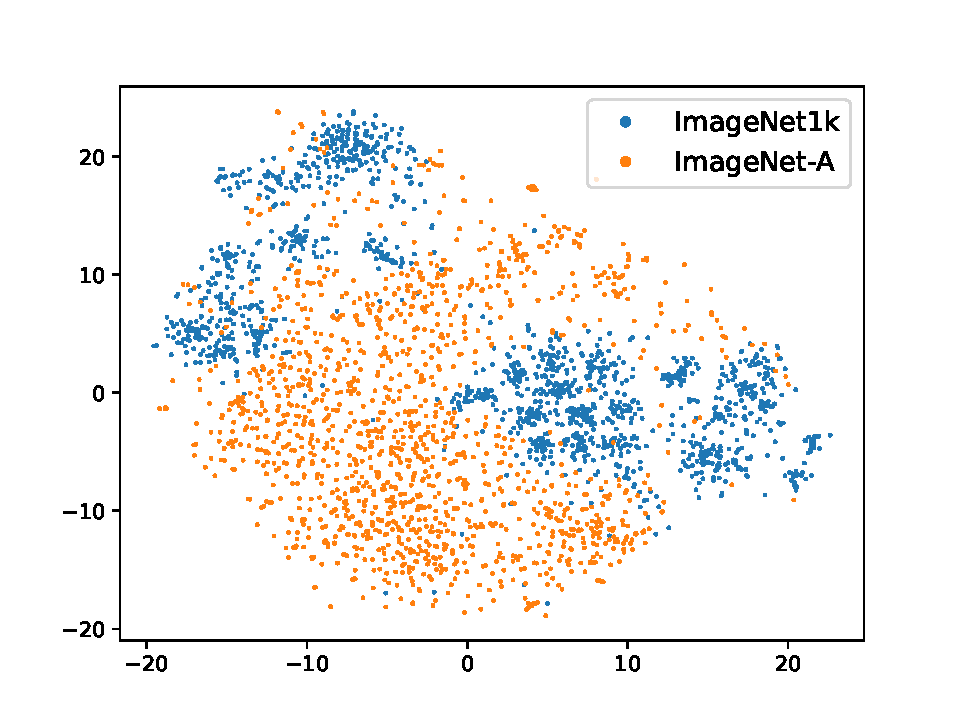
\includegraphics[scale=0.5]{tsne_1k_A.pdf}
\end{figure}

The t-SNE plots should be analyzed carefully because distance or congestion on a t-SNE plot does not always reflect distance or congestion in the original space.
What can be seen from this plot is that the representations are almost separable.
The t-SNE function did not have any information about the datasets the representations belonged to.
The representations could have been mixed up, but they are not, which confirms the observation that OoD detection for this pair of datasets is very successful with the simple baselines.

One more observation is that the set of cosines is pretty stable in a way.
Let us sort all the cosines with all the prototypes in the descending order.
For a particular data point we would get a vector of $K$ values.
If we take a whole dataset, we can compute the mean and variance for every single order statistic.
Then we can compare these means and variances for ID and OoD datasets.
The values of cosines are stable, meaning the standard deviation is very small compared to the mean values.
The plot is at the figure \ref{fig:cosines_1k_A}.
The standard deviations for both datasets are drawn in a semi-transparent colors around the curves slightly seen because they are small.

\begin{figure}[H]
\caption{Distribution of sorted cosines for ID and OoD data points}
\label{fig:cosines_1k_A}
\centering
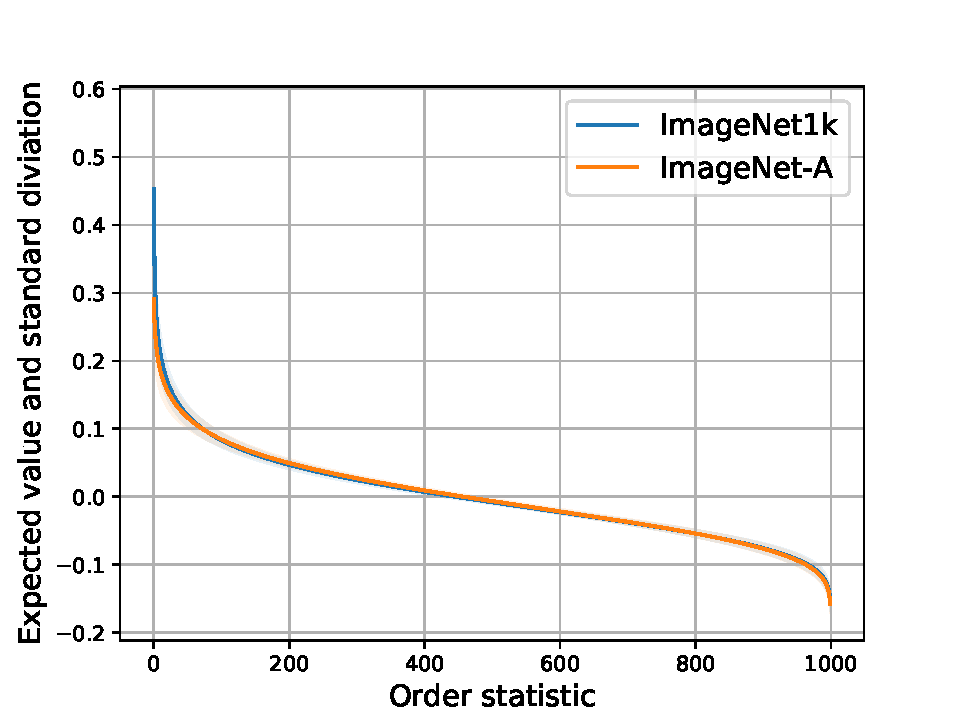
\includegraphics[scale=0.5]{cosines_sorted_mean_ImageNet1k-A.pdf}
\end{figure}

Also the less similar data points are to the training ones, the less is the maximal logit and maximal cosine values.
At the table \ref{table:max_logit_cosine} there is the average value of the maximal logit for the validation set of ImageNet1k and for the five subsets of the ImageNet-C reflecting different corruption levels.

% Table 1
\begin{table}[H]
  \caption{Average maximal logit and average maximal cosine values $\pm \sigma$ for the validation subset of ImageNet1k (corruption level zero) and the subsets of ImageNet-C split by the corruption level (from one to five)}
  \label{table:max_logit_cosine}
  \vskip 0.15in
  \begin{center}
  \begin{small}
    \begin{tabular}{ l | c c c c c c }
      \toprule
      Corruption level & C0 & C1 & C2 & C3 & C4 & C5 \\
      \midrule
      Maximal logit
      & 17.4 {\tiny $\pm$ 4.8} & 14.4 {\tiny $\pm$ 4.6} & 13.1 {\tiny $\pm$ 4.5} & 12.0 {\tiny $\pm$ 4.2} & 10.8 {\tiny $\pm$ 3.7} & 10.0 {\tiny $\pm$ 3.3} \\
      Maximal cosine
      & 0.45 {\tiny $\pm$ 0.11} & 0.38 {\tiny $\pm$ 0.11} & 0.35 {\tiny $\pm$ 0.11} & 0.32 {\tiny $\pm$ 0.1} & 0.29 {\tiny $\pm$ 0.09} & 0.27 {\tiny $\pm$ 0.07} \\
      \bottomrule
    \end{tabular}
  \end{small}
  \end{center}
\end{table}

So with the corruption becoming higher the representations move away from the training representations and the prototypes.
This means the uncertainty measures produced by the simple baselines are able to reflect the level of similarity to the training data.
% ToDo: go on from here

\section{Performance measurement}
\label{section:experiments}
%ToDo: mb you'll want to put it before the analysis section
%ToDo: describe models, datasets, tasks
%ToDo: say results from evidential paper are irreproducible
%ToDo: Compare conventional parametrization with that proposed in the evidential
We show the simple baselines and some modification of the Evidential approach work in the cases close to the real world (i.e., with architectures like ResNet and datasets like ImageNet).
Earlier, the experiments were performed in simple scenarios (e.g., on the MNIST dataset with architectures like LeNet).
As the primary goal of developing such uncertainty estimation methods is to make Machine Learning systems safer, we cannot just take simple experiments as proof of concept.
As there was no explicit mechanism, which explains the ability of the simple baselines to detect OoD samples, we need to be sure these results were not caused by luck and that they can be generalized to more complex cases.
That is why we attempt to validate these methods in large-scale scenarios.
The large scale here means taking large neural networks, large datasets with a large number of classes.

\subsection{Datasets}
We use CIFAR-10, CIFAR-100 \cite{cifar} and ImageNet1k \cite{imagenet} as ID datasets.
ImageNet1k is a subset of the larger dataset ImageNet22k (also referred to as full ImageNet).
There are 1000 classes in the ImageNet1k and 21841 in the ImageNet22k, including the 1000 classes of the ImageNet1k.
If one excludes these 1000 classes from the full ImageNet, one will get the so-called ImageNet21k, which could be used as an OoD dataset for the ImageNet1k because objects from the ImageNet21k are semantically different from the objects from ImageNet1k.

For CIFAR we use SVNH \cite{svhn} and LSUN \cite{lsun} datasets as OoD datasets.
Also, the CIFAR10 and CIFAR100 are both OoD for each other.

For ImageNet1k we use ImageNet21k, ImageNet-A \cite{imagenet_a_o}, ImageNet-O, ImageNet-R \cite{imagenet_r} and ImageNet-C \cite{imagenet_c} as OoD datasets.
The first two consist of natural adversarial examples.
They were gathered by finding the images that would mislead a large network trained on the ImageNet1k.
Images from the ImageNet-A are gathered the way the network provides wrong class labels for underrepresented images of the input domain.
Images from the ImageNet-O are the OoD examples, which a simple baseline (maximal probability) treats as ID.
The last two are the corrupted versions of the ImageNet.
The ImageNet-R is the rendered version of the ImageNet.
The images have a completely different unknown texture, which can harm classification accuracy, although the objects themselves are recognizable but human.
The ImageNet-C contains the validation ImageNet1k set corrupted with 19 different corruptions of five levels of severity each.
So there are 19 times five modifications of the validation subset of the ImageNet1k.
As such, corrupted images do not occur in the ImageNet1k, and they are treated as OoD.

\subsection{Architectures}
We train a Wide ResNet 28-10 \cite{wide_resnet} for CIFAR10 and CIFAR100 and a ResNet 50 \cite{resnet} for ImageNet1k.
All the training details, hyperparameters, and data pre-processing were replicated from the original papers.

\subsection{Picking the best Evidential setting}
We compared different evidential settings presented in the original paper \cite{evidential_classification} and found out the basic cross-entropy network with softmax works better than any other settings.
Here is the performance on the original task of the evidential networks trained with different losses proposed in the original paper.
The regularization was turned on and off to track how it affects the performance for all the losses.
The results are in the table \ref{table:accuracy_evidential}.
The Type II loss refers to the cross-entropy loss, it is just another name used in the original paper.
The last layer activation is exponent instead of the ReLU.
The $L_2$ loss on probabilities shows the worst performance among all the losses.
The regularization makes training complicated, and it affects the performance much worse than the choice of the loss function does.

% Table 2
\begin{table}[H]
  \caption{Validation accuracy (\% $\pm \sigma$) on the original task after training training with evidential losses with and without KL regularization}
  \label{table:accuracy_evidential}
  \vskip 0.15in
  \begin{center}
  \begin{small}
    \begin{tabular}{ l | c c | c c | c c }
      \toprule
      \multirow{2}{*}{Train set} & \multicolumn{2}{c|}{Type II loss} & \multicolumn{2}{c|}{Gibbs classifier's loss} & \multicolumn{2}{c}{$L_2$ loss on probabilities} \\
      & Reg on & Reg off & Reg on & Reg off & Reg on & Reg off \\ \midrule
      CIFAR10
      & 95.2 {\tiny $\pm$ 0.2} & \bf{96.2} {\tiny $\pm$ 0.1}
      & 95.4 {\tiny $\pm$ 0.2} & \bf{96.2} {\tiny $\pm$ 0.1}
      & 18.6 {\tiny $\pm$ 2.7} & \bf{96.1} {\tiny $\pm$ 0.1} \\
      CIFAR100
      & 45.2 {\tiny $\pm$ 0.1} & \bf{81.0} {\tiny $\pm$ 0.3}
      & 31.1 {\tiny $\pm$ 2.7} & \bf{80.9} {\tiny $\pm$ 0.2}
      & 1.0 {\tiny $\pm$ 0.0} & 77.3 {\tiny $\pm$ 0.2} \\
      \bottomrule
    \end{tabular}
  \end{small}
  \end{center}
\end{table}

It turned out that although the choice of the loss function, parametrization, the fact of regularization does not influence the performance of LeNet on MNIST, there is a dramatic difference for a Wide ResNet on CIFAR (especially CIFAR-100).
The ReLU activation made the network very difficult to train possibly due to the death of neurons or maybe because it is just a more difficult optimization problem.
We compared different last layer activation functions including exponent, ReLU and the SoftPlus.
The results of the performance on the base task are in the table \ref{table:last_layer_activation}.
They suggest it is better to use the conventional exponent.

% Table 3
\begin{table}[H]
  \caption{Validation accuracy (\% $\pm \sigma$) on the original task after training using different last layer activations with the type II loss and with no regularization}
  \label{table:last_layer_activation}
  \vskip 0.15in
  \begin{center}
  \begin{small}
    \begin{tabular}{ l | c c c }
      \toprule
      Train dataset & Exponent & ReLU & Softplus \\
      \midrule
      CIFAR10
      & \bf{96.17} {\tiny $\pm$ 0.17} & 59.31 {\tiny $\pm$ 17.78} & 95.79 {\tiny $\pm$ 0.09} \\
      CIFAR100
      & \bf{81.00} {\tiny $\pm$ 0.33} & 32.17 {\tiny $\pm$ 2.90} & 67.3 {\tiny $\pm$ 0.7} \\
      \bottomrule
    \end{tabular}
  \end{small}
  \end{center}
\end{table}

In the table \ref{table:evidential_losses_ood} we present the results of OoD detection performance.
We show that the Type II Maximum Likelihood loss with no regularization can lead to good OoD detection performance.
The accuracy on the base task correlates with the OoD detection performance.
We can also see here and from the table \ref{table:accuracy_evidential} that a basic cross-entropy network with the softmax activation works better for both OoD detection and the base task than any of the original Evidential settings.
For some reason, such experiment was not presented in the original paper.

% Table 4
\begin{table}[H]
  \vskip 0.15in
  \begin{center}
  \caption{OOD detection performance (AUROC \% $\pm \sigma$) using different uncertainty measures for a single evidential model trained with different losses and with or without KL regularization}
  \label{table:evidential_losses_ood}
  \begin{small}
  \begin{tabular}{ l l l | c c c | c c c }
    \toprule
    \multicolumn{2}{c}{Dataset} & \multirow{2}{*}{Reg} & \multicolumn{3}{c |}{EoE} & \multicolumn{3}{c}{MI} \\
    ID & OOD & & Type II & Gibbs & $L_2$ & Type II & Gibbs & $L_2$ \\
    \midrule
    \multirow{8}{*}{C10} & \multirow{2}{*}{SVHN} % CIFAR10 vs SVHN
    & On
    & 92.4 {\tiny $\pm$ 1.6} & 89.7 {\tiny $\pm$ 3.1} & 41.3 {\tiny $\pm$ 9.8}
    & 92.4 {\tiny $\pm$ 1.6} & 90.1 {\tiny $\pm$ 3.1} & 34.0 {\tiny $\pm$ 11.4} \\
    & & Off
    & 94.2 {\tiny $\pm$ 1.4} & 93.6 {\tiny $\pm$ 2.0} & 91.6 {\tiny $\pm$ 3.0}
    & 92.7 {\tiny $\pm$ 2.7} & 91.9 {\tiny $\pm$ 3.0} & 89.6 {\tiny $\pm$ 4.4} \\
    \cmidrule[0.5pt](lr){2-9}
    & \multirow{2}{*}{C100} % CIFAR10 vs CIFAR100
    & On
    & 88.0 {\tiny $\pm$ 0.4} & 87.6 {\tiny $\pm$ 0.5} & 50.6 {\tiny $\pm$ 1.6}
    & 88.0 {\tiny $\pm$ 0.4} & 87.9 {\tiny $\pm$ 0.5} & 50.2 {\tiny $\pm$ 1.3} \\
    & & Off
    & 88.9 {\tiny $\pm$ 0.4} & 88.8 {\tiny $\pm$ 0.4} & 86.3 {\tiny $\pm$ 1.0}
    & 87.2 {\tiny $\pm$ 0.8} & 87.4 {\tiny $\pm$ 0.5} & 84.1 {\tiny $\pm$ 1.6} \\
    \cmidrule[0.5pt](lr){2-9}
    & \multirow{2}{*}{LSUN} % CIFAR10 vs LSUN
    & On
    & 90.6 {\tiny $\pm$ 0.9} & 91.3 {\tiny $\pm$ 0.6} & 54.7 {\tiny $\pm$ 4.6}
    & 90.6 {\tiny $\pm$ 0.9} & 91.4 {\tiny $\pm$ 0.6} & 52.0 {\tiny $\pm$ 4.9} \\
    & & Off
    & 91.2 {\tiny $\pm$ 0.8} & 89.9 {\tiny $\pm$ 1.3} & 88.5 {\tiny $\pm$ 1.7}
    & 90.6 {\tiny $\pm$ 1.2} & 88.5 {\tiny $\pm$ 2.3} & 86.5 {\tiny $\pm$ 2.5} \\
    \cmidrule[0.5pt](lr){2-9}
    & \multirow{2}{*}{TIM} % CIFAR10 vs TinyImageNet
    & On
    & 87.4 {\tiny $\pm$ 0.3} & 87.4 {\tiny $\pm$ 0.3} & 52.2 {\tiny $\pm$ 1.9}
    & 87.4 {\tiny $\pm$ 0.3} & 87.4 {\tiny $\pm$ 0.3} & 51.4 {\tiny $\pm$ 2.4} \\
    & & Off
    & 87.8 {\tiny $\pm$ 0.4} & 87.6 {\tiny $\pm$ 0.3} & 85.5 {\tiny $\pm$ 0.8}
    & 87.1 {\tiny $\pm$ 0.6} & 86.4 {\tiny $\pm$ 0.6} & 83.8 {\tiny $\pm$ 1.1} \\
    \midrule
    \multirow{8}{*}{C100} & \multirow{2}{*}{SVHN} % CIFAR100 vs SVHN
    & On
    & 43.5 {\tiny $\pm$ 6.7}  & 41.8 {\tiny $\pm$ 4.5} & 50.0 {\tiny $\pm$ 0.0}
    & 39.0 {\tiny $\pm$ 11.6} & 47.6 {\tiny $\pm$ 7.8} & 50.0 {\tiny $\pm$ 0.0} \\
    & & Off
    & 79.9 {\tiny $\pm$ 3.9} & 77.2 {\tiny $\pm$ 5.0} & 78.1 {\tiny $\pm$ 3.6}
    & 80.4 {\tiny $\pm$ 5.0} & 77.8 {\tiny $\pm$ 6.3} & 78.8 {\tiny $\pm$ 4.3} \\
    \cmidrule[0.5pt](lr){2-9}
    & \multirow{2}{*}{C10} % CIFAR100 vs CIFAR10
    & On
    & 51.6 {\tiny $\pm$ 1.9} & 59.2 {\tiny $\pm$ 0.6} & 50.0 {\tiny $\pm$ 0.0}
    & 50.6 {\tiny $\pm$ 3.2} & 59.0 {\tiny $\pm$ 0.6} & 50.0 {\tiny $\pm$ 0.0} \\
    & & Off
    & 81.3 {\tiny $\pm$ 1.2} & 81.4 {\tiny $\pm$ 0.8} & 78.2 {\tiny $\pm$ 1.1}
    & 80.8 {\tiny $\pm$ 1.9} & 81.1 {\tiny $\pm$ 1.2} & 77.0 {\tiny $\pm$ 1.7} \\
    \cmidrule[0.5pt](lr){2-9}
    & \multirow{2}{*}{LSUN} % CIFAR100 vs LSUN
    & On
    & 54.3 {\tiny $\pm$ 1.0} & 53.4 {\tiny $\pm$ 2.9} & 50.0 {\tiny $\pm$ 0.0}
    & 56.6 {\tiny $\pm$ 3.2} & 57.2 {\tiny $\pm$ 2.4} & 50.0 {\tiny $\pm$ 0.0} \\
    & & Off
    & 75.5 {\tiny $\pm$ 1.2} & 75.8 {\tiny $\pm$ 1.7} & 71.3 {\tiny $\pm$ 3.0}
    & 74.0 {\tiny $\pm$ 2.1} & 74.8 {\tiny $\pm$ 2.3} & 69.1 {\tiny $\pm$ 4.6} \\
    \cmidrule[0.5pt](lr){2-9}
    & \multirow{2}{*}{TIM} % CIFAR100 vs TinyImageNet
    & On
    & 51.2 {\tiny $\pm$ 0.8} & 58.4 {\tiny $\pm$ 0.8} & 50.0 {\tiny $\pm$ 0.0}
    & 51.2 {\tiny $\pm$ 1.8} & 58.2 {\tiny $\pm$ 1.5} & 50.0 {\tiny $\pm$ 0.0} \\
    & & Off
    & 81.7 {\tiny $\pm$ 0.4} & 81.6 {\tiny $\pm$ 0.4} & 78.6 {\tiny $\pm$ 0.4}
    & 81.1 {\tiny $\pm$ 0.5} & 81.1 {\tiny $\pm$ 0.6} & 76.6 {\tiny $\pm$ 0.7} \\
    \bottomrule
  \end{tabular}
  \end{small}
  \end{center}
\end{table}

\subsection{Classification accuracy of the Cross-Entropy network}
In the table \ref{table:accuracy} there is the top1 accuracy of the models measured on the ID validation set and the corresponding OoD datasets.
Not all OoD datasets were used, only those, which consist of the same classes presented in the training dataset tasks.
The networks were trained with the cross-entropy loss and with the softmax transformation of the logits.
Accuracy for the validation ID sets is the same as reported in the papers describing the networks' architectures.
We can see that the models fail to classify images correctly from ImageNet-A, ImageNet-R, and ImageNet-C as was expected because, for OoD objects, the deep neural networks can not give reliable predictions.

% Table 5
\begin{table}[H]
  \caption{Accuracy (\%) $\pm \sigma$ on the original task after training with cross-entropy loss}
  \label{table:accuracy}
  \vskip 0.15in
  \begin{center}
  \begin{small}
    \begin{tabular}{ l | l | c c }
      \toprule
      Train dataset & Testing dataset & One model & Ensemble \\ \midrule
      CIFAR-10      & CIFAR-10-val    & 96.2 {\tiny $\pm$ 0.2} & \bf{97.0} \\
      CIFAR-100     & CIFAR-100-val   & 81.0 {\tiny $\pm$ 0.3} & \bf{84.5} \\
      \midrule
      \multirow{4}{*}{ImageNet1k} & ImageNet1k-val & 75.9 {\tiny $\pm$ 0.1} & \bf{79.0} \\
      & ImageNet-A & \bf{4.4} {\tiny $\pm$ 0.2} & 3.9 \\
      & ImageNet-R & 35.0 {\tiny $\pm$ 0.2} & \bf{38.8} \\
      & ImageNet-C & 39.1 {\tiny $\pm$ 0.7} & \bf{43.5} \\
      \bottomrule
    \end{tabular}
  \end{small}
  \end{center}
\end{table}

\subsection{OoD detection performance of the Simple baselines}
Here we measure the performance of the simple baselines on OoD detection and compare it with the Deep Ensembles.
If the performance of the baselines is comparable or better than Deep Ensembles', it means the simple baselines are scalable.
Some minor performance drop of the simple baselines is acceptable given the fact that ensembles are better predictors on the base task.
The results are in the table \ref{table:ood_performance}.

% Table 6
\begin{table}[H]
  \begin{center}
  \caption{OOD detection performance (AUROC \% $\pm \sigma$) for a single model trained with cross-entropy loss and an ensemble of ten such models}
  \label{table:ood_performance}
  \begin{small}
  \begin{tabular}{ l l | c | c | c c | c c | c c }
    \toprule
    \multirow{2}{*}{ID set} & \multirow{2}{*}{OOD set} & \multicolumn{1}{c|}{MaxCos} & \multicolumn{1}{c|}{MaxLogit} & \multicolumn{2}{c|}{ExE} & \multicolumn{2}{c|}{MI} & \multicolumn{2}{c}{EPKL} \\
    & & Single & Single & Single & Ens & Single & Ens & Single & Ens \\
    \midrule
    \multirow{3}{*}{CIFAR10}
    & CIFAR100  & \bf{89.2} {\tiny $\pm$ 1.0}
                & 86.7 {\tiny $\pm$ 1.0}
                & 88.9 {\tiny $\pm$ 0.4} & \bf{92.4}
                & 88.1 {\tiny $\pm$ 0.6} & \bf{91.9}
                & 88.3 {\tiny $\pm$ 0.6} & \bf{91.7} \\
    & SVHN      & \bf{95.2} {\tiny $\pm$ 1.2}
                & 93.4 {\tiny $\pm$ 1.8}
                & 94.3 {\tiny $\pm$ 1.4} & \bf{97.4}
                & 94.1 {\tiny $\pm$ 2.0} & \bf{97.2}
                & 94.2 {\tiny $\pm$ 1.9} & 97.0 \\
    & LSUN      & \bf{92.2} {\tiny $\pm$ 1.8}
                & 89.7 {\tiny $\pm$ 1.6}
                & 91.0 {\tiny $\pm$ 0.9} & \bf{94.0}
                & 91.0 {\tiny $\pm$ 1.4} & \bf{92.6}
                & 91.1 {\tiny $\pm$ 1.4} & 92.2 \\
    \midrule
    \multirow{3}{*}{CIFAR100}
    & CIFAR10  & 81.0 {\tiny $\pm$ 0.7}
               & 80.1 {\tiny $\pm$ 1.0}
               & 80.9 {\tiny $\pm$ 0.6} & \bf{84.1}
               & 80.2 {\tiny $\pm$ 0.9} & 80.7
               & 80.2 {\tiny $\pm$ 0.9} & 79.0 \\
    & SVHN     & 77.0 {\tiny $\pm$ 5.2}
               & 78.8 {\tiny $\pm$ 4.7}
               & 79.0 {\tiny $\pm$ 4.6} & 82.6
               & 80.0 {\tiny $\pm$ 4.6} & 81.2
               & 80.0 {\tiny $\pm$ 4.6} & 80.5 \\
    & LSUN     & 76.0 {\tiny $\pm$ 1.2}
               & 75.0 {\tiny $\pm$ 1.7}
               & 76.0 {\tiny $\pm$ 1.4} & 78.4
               & 74.8 {\tiny $\pm$ 2.1} & 76.7
               & 74.9 {\tiny $\pm$ 2.0} & 75.8 \\
    \midrule
    \multirow{8}{*}{ImNet-1k}
    & ImNet-O    & \bf{68.0} {\tiny $\pm$ 0.3} % Max cosine
                 & 57.1 {\tiny $\pm$ 0.3} % MaxLogit
                 & 49.5 {\tiny $\pm$ 0.3} & \bf{51.8} % ExE
                 & 57.4 {\tiny $\pm$ 0.4} & \bf{60.9} % MI
                 & 58.1 {\tiny $\pm$ 0.4} & \bf{63.5} \\ % EPKL
    & ImNet-A    & \bf{88.1} {\tiny $\pm$ 0.1} % Max cosine
                 & 86.3 {\tiny $\pm$ 0.2} % MaxLogit
                 & 86.5 {\tiny $\pm$ 0.1} & \bf{88.8} % ExE
                 & 85.7 {\tiny $\pm$ 0.2} & \bf{87.0} % MI
                 & 85.8 {\tiny $\pm$ 0.2} & 85.8 \\ % EPKL
    & ImNet-R    & \bf{87.1} {\tiny $\pm$ 0.2} % Max cosine
                 & 85.5 {\tiny $\pm$ 0.2} % MaxLogit
                 & 83.1 {\tiny $\pm$ 0.2} & \bf{85.6} % ExE
                 & \bf{86.1} {\tiny $\pm$ 0.2} & 84.8 % MI
                 & \bf{86.2} {\tiny $\pm$ 0.2} & 84.1 \\ % EPKL
    & ImNet-C1   & 66.7 {\tiny $\pm$ 0.2} % Max cosine
                 & \bf{68.0} {\tiny $\pm$ 0.3} % MaxLogit
                 & 66.5 {\tiny $\pm$ 0.2} & \bf{67.9} % ExE
                 & 67.9 {\tiny $\pm$ 0.3} & 67.3 % MI
                 & \bf{68.1} {\tiny $\pm$ 0.3} & 67.1 \\ % EPKL
    & ImNet-C2   & 74.6 {\tiny $\pm$ 0.3} % Max cosine
                 & \bf{75.4} {\tiny $\pm$ 0.4} % MaxLogit
                 & 73.8 {\tiny $\pm$ 0.3} & \bf{75.8} % ExE
                 & 75.3 {\tiny $\pm$ 0.4} & 75.4 % MI
                 & 75.4 {\tiny $\pm$ 0.4} & 75.1 \\ % EPKL
    & ImNet-C3   & 80.5 {\tiny $\pm$ 0.3} % Max cosine
                 & \bf{81.2} {\tiny $\pm$ 0.4} % MaxLogit
                 & 79.4 {\tiny $\pm$ 0.3} & \bf{81.7} % ExE
                 & 81.1 {\tiny $\pm$ 0.5} & 81.0 % MI
                 & 81.2 {\tiny $\pm$ 0.5} & 80.5 \\ % EPKL
    & ImNet-C4   & 86.4 {\tiny $\pm$ 0.2} % Max cosine
                 & \bf{87.2} {\tiny $\pm$ 0.3} % MaxLogit
                 & 85.3 {\tiny $\pm$ 0.2} & \bf{87.7} % ExE
                 & \bf{87.3} {\tiny $\pm$ 0.3} & 86.0 % MI
                 & \bf{87.3} {\tiny $\pm$ 0.3} & 85.2 \\ % EPKL
    & ImNet-C5   & 90.6 {\tiny $\pm$ 0.2} % Max cosine
                 & \bf{91.5} {\tiny $\pm$ 0.3} % MaxLogit
                 & 89.6 {\tiny $\pm$ 0.3} & \bf{91.9} % ExE
                 & \bf{91.6} {\tiny $\pm$ 0.3} & 88.4 % MI
                 & \bf{91.6} {\tiny $\pm$ 0.3} & 87.3 \\ % EPKL
    \bottomrule
  \end{tabular}
  \end{small}
  \end{center}
\end{table}

We can see that the Expected Pairwise KL-Divergence (EPKL) of the Dirichlet of a single cross-entropy model (i.e., exactly an evidential model without regularization) works on par with the EPKL of a Deep Ensemble.
The EPKL, as well as the Mutual Information (MI), in the context of ensembles, measures the disagreement of different models in the ensemble.
In the context of Dirichlet-based models, mutual information and EPKL measure sharpness of the Dirichlet distribution and depend on the parameters that were inferred from the model: the higher the parameters are, the sharper the distribution is.
The Expected Entropy (ExE) of a single model is just the entropy of the softmax.
It is also a good baseline for the OoD detection task.
Here we can see that the simple baselines perform on par with the conventional Deep Ensembles' mutual information and sometimes the baselines.
We can also see that the newly proposed maximal cosine and the maximal logit are very good baselines.
The maximal logit of a single model outperforms the ensemble's EPKL on almost all of the ImageNet's OoD datasets except ImageNet-O.
All the methods work poorly on ImageNet-O, most likely because it consists of adversarial samples gathered the way they full one of the simple baselines (i.e., maximal probability).

\section{Conclusions}
\label{section:conclusion}
We have conducted a theoretical and empirical investigation of the behavior of such methods of epistemic uncertainty estimation like the Evidential Networks and simple baselines like maximal logit and the entropy of softmax for widely used neural networks architectures in computer vision.
We have tested the approaches on large-scale tasks and showed that the Evidential setting proposed in the original paper does not scale up.
However, a simple modification to this setting scales up very well and provides good performance on Out-of-Distribution (OoD) detection tasks.
We have also shown the connection of these methods with the distance-based approaches by introducing a kernel function, which maps representations of the penultimate layer of a classification neural network to scalars, which are then interpreted as estimates of epistemic uncertainty.
We have introduced a new method of epistemic uncertainty estimation (maximal cosine between the penultimate layer representations and the prototypes of the classes) and showed that it works on par with similar uncertainty estimation baselines.
We also showed that some uncertainty estimation baselines like the maximal cosine and the maximal logit reflect the similarity of the testing object to the training ones. The less an object is similar to the training ones, the higher is the level of uncertainty.

\newpage
\bibliography{references}
\bibliographystyle{apalike}
% ToDo: check that references are in the end of the document

\end{document}